\documentclass{article}
\usepackage[spanish]{babel}
\usepackage[utf8]{inputenc}
\usepackage{amsmath}
\usepackage{amsthm}
\usepackage{amsfonts}
\usepackage{graphicx}
\newtheorem{mydef}{Definition}
\newtheorem{mythm}{Theorem}
\newtheorem{myprf}{Proof}
\title{Práctica 1}
\author{Justo Andrés Manrique Urbina}
\begin{document}
\maketitle
\section{Análisis descriptivo de los datos}
\subsection{Análisis de variables categóricas}
Se realizó un análisis univariado de las variables categóricas, a fin de observar la distribución de la base de datos en relación a dichas variables. Se observó lo siguiente:
\begin{itemize}
	\item Se observa que el departamento con menos casos y más casos es Callao y Lima respectivamente.
	\item Se observa que los quintiles de riqueza se mantienen constantes a lo largo de la muestra observada.
	\item Se observa que existen preponderancia de dos instituciones en la muestra observada (aproximadamente 12 mil observaciones corresponden a las instituciones 1 y 2), mientras que el resto proviene de las instituciones de 3 y 4.
	\item Se observa preponderancia de un idioma (aproximadamente 12 mil observaciones) frente a los otros dos.
\end{itemize}
\subsection{Análisis de variables continuas}
Se realizó una matriz de dispersión sobre las variables continuas para observar el grado de relación lineal que las covariables tienen con la variable respuesta. En base a ello, se observó lo siguiente:
\begin{itemize}
	\item El tiempo de llegada tiene una relación lineal negativa con la variable respuesta. El grado de dicha relación lineal es medianamente fuerte (mayor a 0.5). No obstante, se observó que el tiempo de llegada es bimodal, lo cual es un indicador de que dicha variable tiene distribución mixta.
	\item El gasto por consulta médica (variable C1P23) parece no tener efecto lineal con la variable respuesta, sin embargo se observa que existen valores muy altos que podrían alterar la relación.
	\item Similarmente, el gasto por traslado al establecimiento de salud (variable C1P9) parece no tener efecto lineal con la variable respuesta, sin embargo se observa que existen valores muy altos que podrían alterar la relación.
\end{itemize}

\begin{figure}
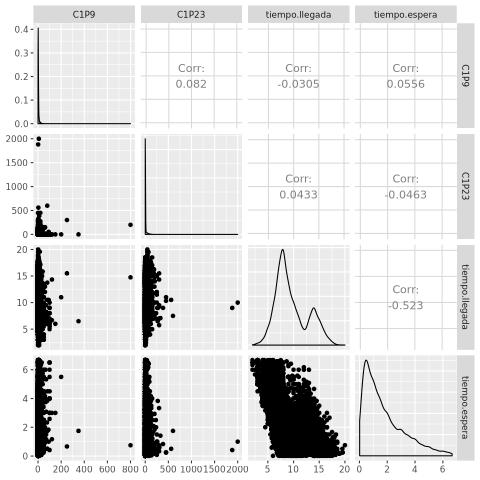
\includegraphics[width=\textwidth]{scatterplot.jpg}
\caption{Análisis de variables continuas}
\label{fig:scp1}
\end{figure}

\section{Selección de variables}
Se utilizó el método LASSO para selección de variables. Para ello, se utilizó la función glmnet con el $\lambda$ mínimo, observando lo siguiente:

\begin{center}
\begin{tabular}{cc}
\hline
Variable        & Valor \\ \hline
Intercepto      & 0.655 \\
Departamento    & 0.06  \\
Institución     & .     \\
C1Turno         & 0.02  \\
C1P77           & 0.55  \\
C1P5            & .     \\
C1P9            & 0.68  \\
C2P23           & .     \\
C1P30           & 0.12  \\
C1P56           & .     \\
C1P80           & 0.10  \\
C1IndiceRiqueza & 0.38  \\
tiempo.llegada  & 0.01  \\ \hline
\end{tabular}
\end{center}

Se utilizó el método stepwise para selección de variables, observando lo siguiente:

\begin{center}
\begin{tabular}{cc}
\hline
Variable       & AIC    \\ \hline
Intercepto     & -893.0 \\
C1P23          & -890.9 \\
C1P9           & -864.6 \\
C1P5           & -587.4 \\
Departamento   & -306.8 \\
Institución    & 25.2   \\
C1Turno        & 2520.0 \\
tiempo.llegada & 5016.1 \\ \hline
\end{tabular}
\end{center}

Se observa que ambos métodos de selección de variable tienen en común las siguientes variables: C1Turno, Departamento, tiempo.llegada, C1P9 (gasto médico por consulta). Sin embargo, estas son las diferencias:
\begin{itemize}
	\item El método LASSO tiene más variables que el método stepwise. Se observa que en total el método LASSO tiene 8 variables, mientras que el método stepwise tiene 7.
	\item El método LASSO considera las variables C1IndiceRiqueza, C1P77, C1P30 y C1P80 dentro de su selección de variables, mientras que el método stepwise no.
	\item El método stepwise considera las variables C1P32, C1P5 e Institución dentro de la selección final de variables, mientras que el método LASSO no.
\end{itemize}
\section{Selección de modelo}
En base a lo anterior, se realizó el siguiente modelo:
\begin{center}
tiempo.espera $~$ C1P23 $+$ C1P9 $+$ C1P5 $+$ Departamento $+$ Institución $+$ C1Turno $+$ tiempo.llegada.
\end{center}

Se realizaron los siguientes análisis de diagnóstico:
\subsection{Normalidad de errores}
Se realizó el qqPlot del modelo, observándose que los residuales podrían seguir una distribución normal, con ligeras variaciones en las colas de la distribución. Ver gráfico a continuación:

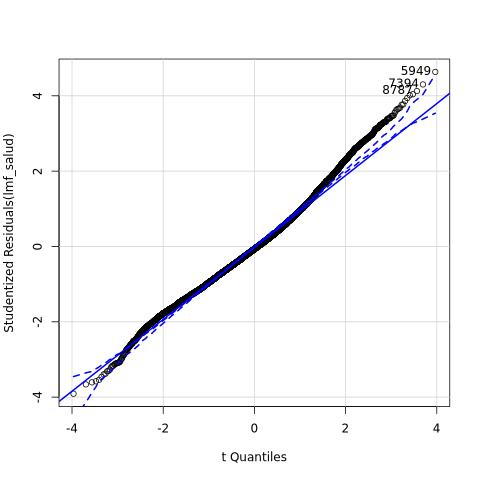
\includegraphics[width=\textwidth]{lm_qqplot.jpg}

\subsection{Valores influyentes}
Se observó que existen valores influyentes en el modeloSe observó que existen valores influyentes en el modelo, como las observaciones 8391,3742, 5949, 7394. Ver gráfico a continuación:

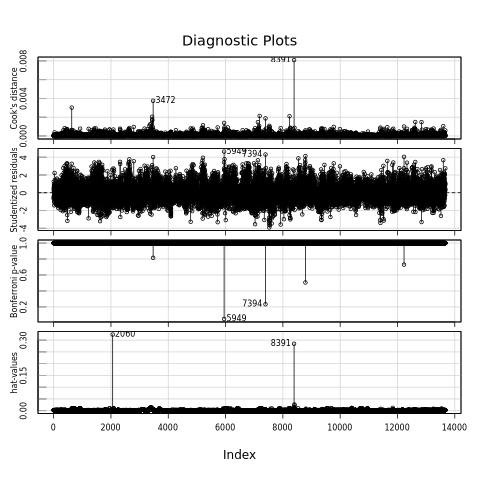
\includegraphics[width=\textwidth]{lm_outliers.jpg}

\subsection{Análisis de varianza}
Se observó que existen la varianza de los residuales no sigue un patrón lineal y es heterocedástica. Al investigar más sobre ello, se observó que el tiempo de llegada contribuye a dicha no linealidad. Ver a continuación la matriz de residuales vs. cada variable:

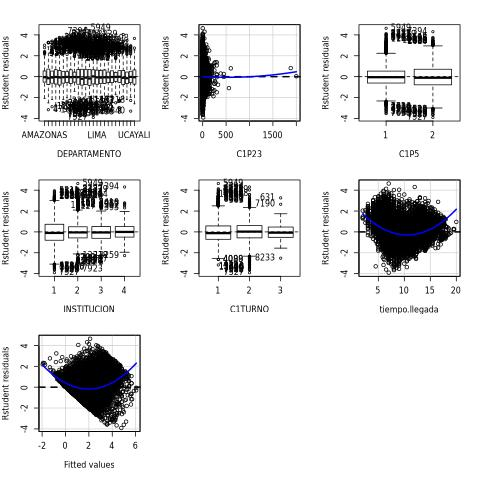
\includegraphics[width=\textwidth]{lm_residuales.jpg}

Cabe resaltar que se observó que los residuales estudentizados del modelo versus los valores ajustados aumentan en la medida que los valores ajustados aumentan por lo que la varianza es heterocedástica. Por lo tanto, se sugiere modelar el tiempo de espera mediante otra distribución.

Con el propósito de controlar la varianza, se propuso aplicarle logaritmo al tiempo de llegada. Sin embargo, se observó que los residuales mantienen la misma forma de cono, por lo que se mantiene la sugerencia de modelar el tiempo de espera mediante otra distribución. Ver a continuación gráfico de los residuales:

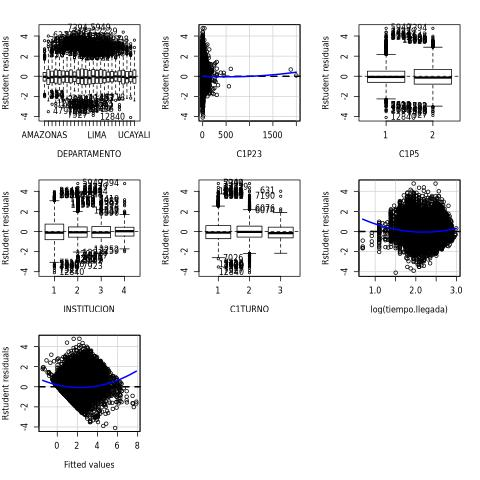
\includegraphics[width=\textwidth]{lm_1_residuales.jpg}

\subsection{Interpretación del modelo}

Ver a continuación los coeficientes del modelo:

\begin{tabular}{@{\extracolsep{5pt}}lc}
\\[-1.8ex]\hline
\hline \\[-1.8ex]
 & \multicolumn{1}{c}{\textit{Dependent variable:}} \\
\cline{2-2}
\\[-1.8ex] & tiempo.espera \\
\hline \\[-1.8ex]
 DEPARTAMENTOANCASH & 0.091 \\
 DEPARTAMENTOAPURIMAC & $-$0.110$^{*}$ \\
 DEPARTAMENTOAREQUIPA & $-$0.277$^{***}$ \\
 DEPARTAMENTOAYACUCHO & $-$0.115$^{*}$ \\
 DEPARTAMENTOCAJAMARCA & $-$0.074 \\
 DEPARTAMENTOCALLAO & $-$0.637$^{***}$ \\
 DEPARTAMENTOCUSCO & 0.091 \\
 DEPARTAMENTOHUANCAVELICA & $-$0.506$^{***}$ \\
 DEPARTAMENTOHUANUCO & 0.080 \\
 DEPARTAMENTOICA & $-$0.133$^{**}$ \\
 DEPARTAMENTOJUNIN & 0.154$^{***}$ \\
 DEPARTAMENTOLA LIBERTAD & 0.009 \\
 DEPARTAMENTOLAMBAYEQUE & 0.102$^{*}$ \\
 DEPARTAMENTOLIMA & $-$0.153$^{***}$ \\
 DEPARTAMENTOLORETO & $-$0.260$^{***}$ \\
 DEPARTAMENTOMADRE DE DIOS & $-$0.287$^{***}$ \\
 DEPARTAMENTOMOQUEGUA & $-$0.041 \\
 DEPARTAMENTOPASCO & $-$0.055 \\
 DEPARTAMENTOPIURA & $-$0.434$^{***}$ \\
 DEPARTAMENTOPUNO & $-$0.398$^{***}$ \\
 DEPARTAMENTOSAN MARTIN & $-$0.092 \\
 DEPARTAMENTOTACNA & $-$0.090 \\
 DEPARTAMENTOTUMBES & $-$0.162$^{**}$ \\
 DEPARTAMENTOUCAYALI & $-$0.416$^{***}$ \\
 C1P23 & $-$0.0004 \\
 C1P52 & 0.299$^{***}$ \\
 INSTITUCION2 & $-$0.503$^{***}$ \\
 INSTITUCION3 & $-$0.608$^{***}$ \\
 INSTITUCION4 & $-$0.822$^{***}$ \\
 C1TURNO2 & 1.628$^{***}$ \\
 C1TURNO3 & 2.630$^{***}$ \\
 log(tiempo.llegada) & $-$3.928$^{***}$ \\
 Constant & 10.198$^{***}$ \\
\hline \\[-1.8ex]
Observations & 13,670 \\
R$^{2}$ & 0.598 \\
Adjusted R$^{2}$ & 0.597 \\
Residual Std. Error & 0.919 (df = 13637) \\
F Statistic & 634.492$^{***}$ (df = 32; 13637) \\
\hline
\hline \\[-1.8ex]
\textit{Note:}  & \multicolumn{1}{r}{$^{*}$p$<$0.1; $^{**}$p$<$0.05; $^{***}
$p$<$0.01} \\
\end{tabular}
\\
En base a la regresión, se observa lo siguiente:
\begin{itemize}
	\item Tomando el departamento Amazonas como referencia, el tiempo de espera es menor para los siguientes departamentos: Apurimac, Arequipa, Ayacucho, Callao, Huancavelica, Ica, Lima, Loreto, Madre de Dios, Piura, Puno, Tumbes, Ucayali. Si la persona se atiende en el departamento de Junín, se espera que el tiempo de espera sea mayor que si fuera atendida en Amazonas. 
	\item Se espera que el gasto por consulta médica no tenga relación con el tiempo de espera (variable C1P23). Asimismo, dicha relación se considera no significativa.
	\item Tomando la institución de categoría 1 como referencia, en la medida que se sube de categoría el tiempo de espera es menor. Ver coeficientes en la tabla.
	\item Se observa también que, tomando el turno de categoría 1 como referencia, en la medida que se sube de categoría se espera que el tiempo de espera sea mayor. Ver coeficientes en la tabla.
	\item Se observa que, en la medida que aumente el logaritmo del tiempo de llegada en una unidad, se espere que el tiempo de llegada se reduzca en 3.928 unidades.
	\item Se observa que el modelo en general es estadísticamente significativo, con un valor F de 639.492.

\end{itemize}

\subsection{Re-estimación del modelo}
Se re-estimó el modelo en base a la función indicadora, obteniéndose lo siguiente:

\begin{itemize}
	\item La varianza parece ser homocedástica, sin embargo se observa que la varianza de los residuos aumenta en la medida que los valores predichos aumentan. Esto es un posible indicador que la distribución normal no es el mejor modelo para este tipo de variable. Ver gráfico de matriz de residuales, en donde en el segundo gráfico de la tercera fila es los residuales estudentizados de los valores ajustados.
\end{itemize}

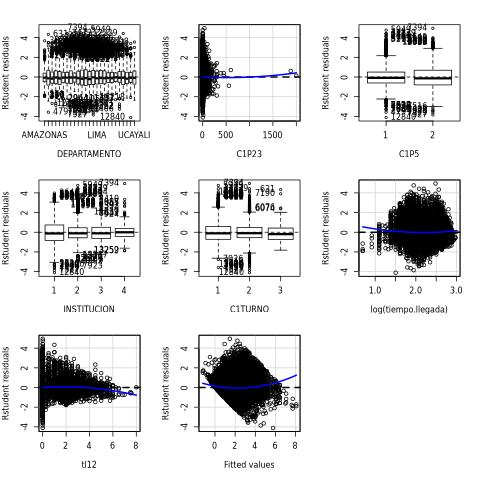
\includegraphics[width=\textwidth]{mf_residuales.jpg}

Ver modelo a continuación:

\begin{tabular}{@{\extracolsep{5pt}}lc}
\\[-1.8ex]\hline
\hline \\[-1.8ex]
 & \multicolumn{1}{c}{\textit{Dependent variable:}} \\
\cline{2-2}
\\[-1.8ex] & tiempo.espera \\
\hline \\[-1.8ex]
 DEPARTAMENTOANCASH & 0.119$^{**}$ \\
 DEPARTAMENTOAPURIMAC & $-$0.088 \\
 DEPARTAMENTOAREQUIPA & $-$0.231$^{***}$ \\
 DEPARTAMENTOAYACUCHO & $-$0.090 \\
 DEPARTAMENTOCAJAMARCA & $-$0.054 \\
 DEPARTAMENTOCALLAO & $-$0.582$^{***}$ \\
 DEPARTAMENTOCUSCO & 0.114$^{**}$ \\
 DEPARTAMENTOHUANCAVELICA & $-$0.470$^{***}$ \\
 DEPARTAMENTOHUANUCO & 0.107$^{*}$ \\
 DEPARTAMENTOICA & $-$0.079 \\
 DEPARTAMENTOJUNIN & 0.193$^{***}$ \\
 DEPARTAMENTOLA LIBERTAD & 0.027 \\
 DEPARTAMENTOLAMBAYEQUE & 0.150$^{**}$ \\
 DEPARTAMENTOLIMA & $-$0.103$^{**}$ \\
 DEPARTAMENTOLORETO & $-$0.230$^{***}$ \\
 DEPARTAMENTOMADRE DE DIOS & $-$0.265$^{***}$ \\
 DEPARTAMENTOMOQUEGUA & $-$0.006 \\
 DEPARTAMENTOPASCO & $-$0.035 \\
 DEPARTAMENTOPIURA & $-$0.377$^{***}$ \\
 DEPARTAMENTOPUNO & $-$0.348$^{***}$ \\
 DEPARTAMENTOSAN MARTIN & $-$0.053 \\
 DEPARTAMENTOTACNA & $-$0.047 \\
 DEPARTAMENTOTUMBES & $-$0.141$^{**}$ \\
 DEPARTAMENTOUCAYALI & $-$0.388$^{***}$ \\
 C1P23 & $-$0.0003 \\
 C1P52 & 0.292$^{***}$ \\
 INSTITUCION2 & $-$0.502$^{***}$ \\
 INSTITUCION3 & $-$0.594$^{***}$ \\
 INSTITUCION4 & $-$0.844$^{***}$ \\
 C1TURNO2 & 1.554$^{***}$ \\
 C1TURNO3 & 2.333$^{***}$ \\
 log(tiempo.llegada) & $-$4.088$^{***}$ \\
 tl12 & 0.094$^{***}$ \\
 Constant & 10.493$^{***}$ \\
\hline \\[-1.8ex]
Observations & 13,670 \\
R$^{2}$ & 0.600 \\
Adjusted R$^{2}$ & 0.599 \\
Residual Std. Error & 0.917 (df = 13636) \\
F Statistic & 620.682$^{***}$ (df = 33; 13636) \\
\hline
\hline \\[-1.8ex]
\textit{Note:}  & \multicolumn{1}{r}{$^{*}$p$<$0.1; $^{**}$p$<$0.05; $^{***}
$p$<$0.01} \\
\end{tabular}

La función indicador se enuncia como \textbf{tl12}. Se puede apreciar en el modelo que, si el tiempo de llegada del paciente es en la tarde (e incremente en una unidad en esa franja de tiempo), aumente el tiempo de espera en 0.094 unidades. Sin embargo, se observa que el efecto de que el tiempo de llegada aumentó de 3.928 a 4.088 por lo que el efecto sigue siendo negativo.
\end{document}
